\chapter{Background}

\section{Memory Management in Native Systems}
Memory management in non-virtualized native multiprogramming system is achieved using Virtual
Memory. In multiprogrammed systems several programs are resident in memory at the same time.
The memory management policy in such a system deals with protecting the memory of one program from 
another, loading a program into available space in main memory, de/allocating memory dynamically
from/to programs.\\
While programs are complied and linked with addresses starting at $0$ and CPU uses 
these addresses to access the binary, it isn't necessary (and is the not the case that) that a
program will get physical memory with the same addresses or it is not even guaranteed that there
will be enough space in the physical memory to load the entire binary of the program. Most of the
times only the immediately needed part of the program is loaded onto the available physical
memory, (the rest will be held in a backing store - often the hard disk) and they will share the
physical memory space along with parts of other programs. And the OS may choose to evict parts of
the program to the backing store when in need of memory as a part of its memory management policy.
Therefore the addresses generated by CPU needs to be translated into the corresponding physical
addresses. The address generated by CPU is called \textit{Virtual Address} or VA . Thus we need to
have a mechanism of \textit{Virtual Address (VA)} $\rightarrow$ \textit{Physical Address (PA)}
translation.\\
Hence the illusion that is given to a program that there is enough physical memory available to
store its entire binary combined with relocation of code having contiguous virtual addresses into
- not necessarily contiguous - available physical memory chunks are the central ideas of virtual
memory.\\
Virtual Memory can be implemented in more than one ways. Paging is one of them. The idea behind
paging is to divide the virtual address space and the physical memory into same sized units of
allocation called \textit{pages}. Hence the virtual address space is divided into \textit{virtual
pages} or simply \textit{pages} and physical memory into \textit{physical pages} or
\textit{frames} or \textit{physical/machine frames}. It is thus clear that not all pages of a
program will be present in the physical memory when the program is executing, the contiguous
virtual pages belonging to the same program needn't be allocated contiguous frames and it is
necessary to provide a way to map from the virtual pages to the associated machine frames.\\
This mapping should be there for each program and this mapping is called the \textit{page table}.
The organisation of page table is closely tied to the size of a page or a frame. Page size is
taken as \textit{power of 2} as this ensures that all binary representable addresses can be
utilized and address manipulation can be done without arithmetic operations. There should an be an
entry for all virtual page addresses of a program in its page table. This will result in a very
long (large) page table and all the page tables of all programs that are currently resident in
memory will consume considerable amount of physical memory. So instead of storing such a single
large page table per program in memory we break the page tables into different levels to have a
tree like structure. Thus following the design principles of virtual memory it is not necessary
that even all the levels of the page table will be resident in memory all the time.\\
Often the entries in each level are grouped into different sets. And each entry will contain a
physical address and some flag bits. The flag bits store permissions and other info about the this
entry and the physical address in the entry points to a set of entries in the next level. These
sets of entries in each level are often limited to single physical frame. Thus the physical
address in a page table entry points to a physical frame in the next level. There is an exception
for the last level of the page table. An entry in the last level contains the physical address of
the actual virtual page that we were looking for and the flag bits of the entry include
information like whether the physical page it points to is present or not. The physical address of
the root of the page table (i.e. the physical address of the base of the outermost level of page
table) is stored in a hardware register.\\
The translation of virtual address to physical address happens in the following manner:\\
The base address of the program's page table is obtained from the hardware register storing it. To
this base address we add that part of the virtual address that corresponds to the outermost level. 
Thus we get the corresponding entry in the outer most level which points to the base address of
the corresponding set of entries of the next level (i.e. a physical page of the next level) . Now
to get to the corresponding entry within that physical page we add the part of virtual address for
the next level to the physical page address we obtained from the outermost level. This process is
continued till we get to a last level entry from which we get the physical frame address 
corresponding to the virtual address. And to go to the exact physical address location
corresponding to the virtual address location add the last part of the virtual that doesn't
correspond to any page table level i.e. the offset part to the physical frame address.\\    
Hence it is clear from the above discussion that the parts of the virtual address that correspond
to each level of page table give us an offset within that level and last part of the virtual
address that doesn't correspond to any page table level gives us the offset within the actual
frame that holds this virtual address. Illustration in figure ~\ref{fig:fig1}.\\
For a virtual address generated by the CPU the translation to physical address i.e. traversing the
levels of page table happens in hardware. If the corresponding physical page is present in the
translated location it is a \textit{hit} else it is a \textit{fault}. Page faults are to be
resolved by moving in the corresponding missing page from the backing store. Certain architectures
like x86 choose to cache recently accessed virtual addresses and their mappings in a small cache
often called the \textit{translational look ahead buffer} or TLB, this is for faster translations
the next the same address is accessed. This also brings about the need for coherence between the
entries in the TLB and the page table. The hardware that does all this is called the
\textit{memory management unit} or MMU.\\
Linux OS on x86 (i.e. 32 bit) architecture has 3 levels of the page table. While for x86\_64 (i.e.
64bit) it has 4. They are called \textit{page global directory} or PGD, \textit{page upper
directory} or PUD, \textit{page middle directory} or PMD and \textit{page table entry} or PTE. x86
won't have the PMD. The \textit{CR3} register holds the base address of the PGD.\\
\begin{figure}[tbp]
  \begin{center}
    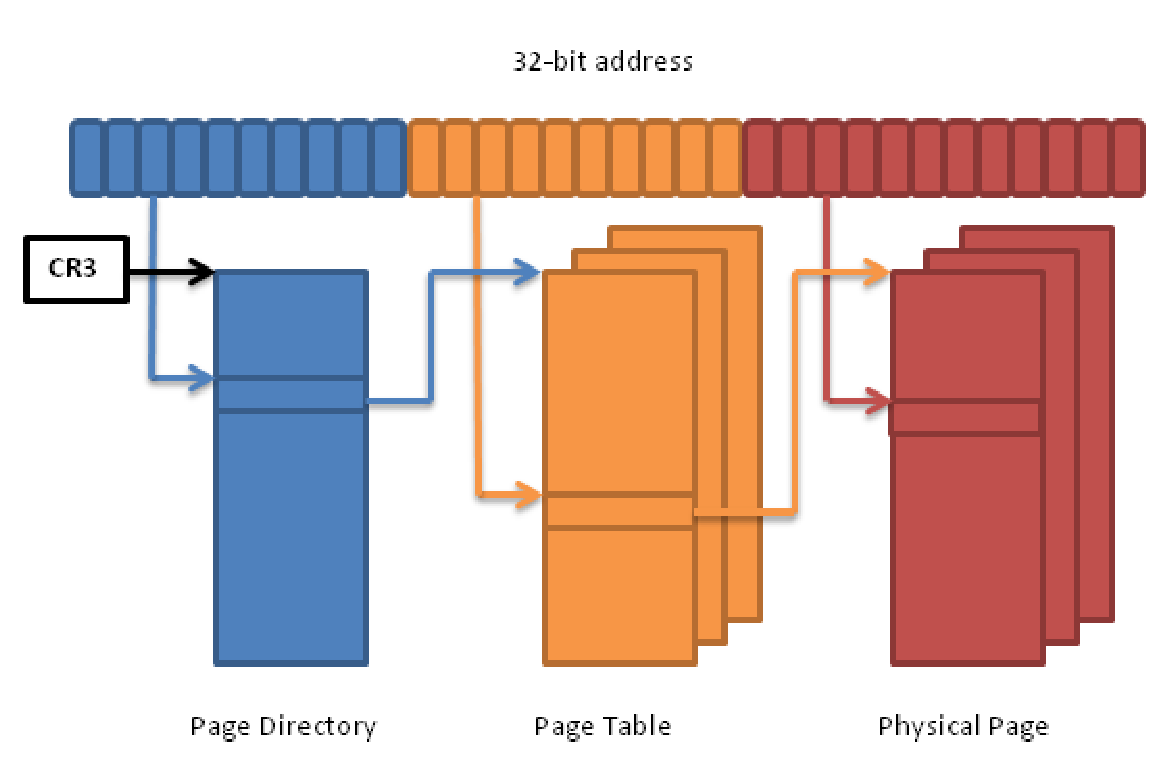
\includegraphics[width=0.7\textwidth]{pagetable}
    \caption[Page Table Illustration]{Illustration of \textit{VA} $\rightarrow$ \textit{PA} address translation.}
    \label{fig:fig1}
  \end{center}
\end{figure}

